% This file was created with tikzplotlib v0.10.1.
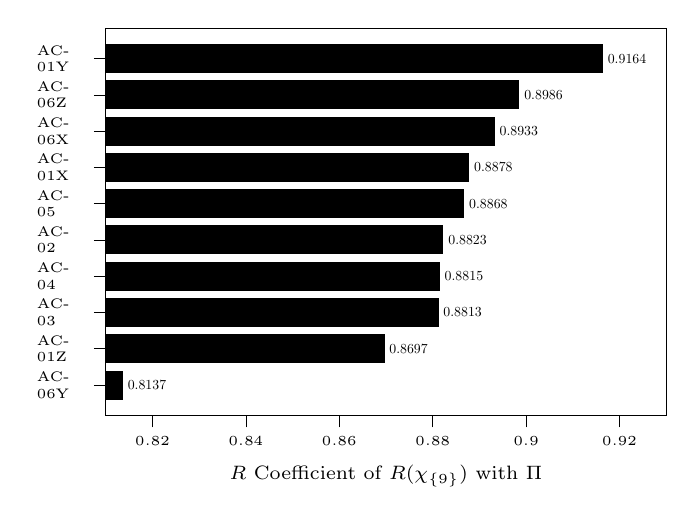
\begin{tikzpicture}

\definecolor{darkgray176}{RGB}{176,176,176}
\definecolor{sienna1279963}{RGB}{127,99,63}
\pgfplotsset{every tick label/.append style={font=\tiny}}

\begin{axis}[
tick align=outside,
tick pos=left,
x grid style={darkgray176},
xlabel={\scriptsize {$R$ Coefficient of $\mathbb{R}(\boldsymbol{\chi}_{\{ 9 \}})$ with $\Pi$}},
xmin=0.81, xmax=0.93,
xtick style={color=black},
y grid style={darkgray176},
ymin=-0.84, ymax=9.84,
ytick style={color=black},
ytick = {0, 1, 2, 3, 4, 5, 6, 7, 8, 9},
yticklabels= {
\parbox{6mm}{AC-06Y},
\parbox{6mm}{AC-01Z},
\parbox{6mm}{AC-03 }, 
\parbox{6mm}{AC-04 }, 
\parbox{6mm}{AC-02 }, 
\parbox{6mm}{AC-05 }, 
\parbox{6mm}{AC-01X}, 
\parbox{6mm}{AC-06X}, 
\parbox{6mm}{AC-06Z}, 
\parbox{6mm}{AC-01Y}, 
},
height=65mm,
width=87mm,
]
\draw[draw=none,fill=black] (axis cs:0,-0.4) rectangle (axis cs:0.813676002547862,0.4);
\draw[draw=none,fill=black] (axis cs:0,0.6)  rectangle (axis cs:0.869683664287886,1.4);
\draw[draw=none,fill=black] (axis cs:0,1.6)  rectangle (axis cs:0.881251568666529,2.4);
\draw[draw=none,fill=black] (axis cs:0,2.6)  rectangle (axis cs:0.881532240479358,3.4);
\draw[draw=none,fill=black] (axis cs:0,3.6)  rectangle (axis cs:0.882312767527318,4.4);
\draw[draw=none,fill=black] (axis cs:0,4.6)  rectangle (axis cs:0.886772687275304,5.4);
\draw[draw=none,fill=black] (axis cs:0,5.6)  rectangle (axis cs:0.887845349607805,6.4);
\draw[draw=none,fill=black] (axis cs:0,6.6)  rectangle (axis cs:0.893280103396994,7.4);
\draw[draw=none,fill=black] (axis cs:0,7.6)  rectangle (axis cs:0.898571596447509,8.4);
\draw[draw=none,fill=black] (axis cs:0,8.6)  rectangle (axis cs:0.916447753679063,9.4);
\draw (axis cs:0.813676002547862,0) ++(0pt,0pt) node[
  scale=0.5,
  anchor=west,
  text=black,
  rotate=0.0
]{0.8137};
\draw (axis cs:0.869683664287886,1) ++(0pt,0pt) node[
  scale=0.5,
  anchor=west,
  text=black,
  rotate=0.0
]{0.8697};
\draw (axis cs:0.881251568666529,2) ++(0pt,0pt) node[
  scale=0.5,
  anchor=west,
  text=black,
  rotate=0.0
]{0.8813};
\draw (axis cs:0.881532240479358,3) ++(0pt,0pt) node[
  scale=0.5,
  anchor=west,
  text=black,
  rotate=0.0
]{0.8815};
\draw (axis cs:0.882312767527318,4) ++(0pt,0pt) node[
  scale=0.5,
  anchor=west,
  text=black,
  rotate=0.0
]{0.8823};
\draw (axis cs:0.886772687275304,5) ++(0pt,0pt) node[
  scale=0.5,
  anchor=west,
  text=black,
  rotate=0.0
]{0.8868};
\draw (axis cs:0.887845349607805,6) ++(0pt,0pt) node[
  scale=0.5,
  anchor=west,
  text=black,
  rotate=0.0
]{0.8878};
\draw (axis cs:0.893280103396994,7) ++(0pt,0pt) node[
  scale=0.5,
  anchor=west,
  text=black,
  rotate=0.0
]{0.8933};
\draw (axis cs:0.898571596447509,8) ++(0pt,0pt) node[
  scale=0.5,
  anchor=west,
  text=black,
  rotate=0.0
]{0.8986};
\draw (axis cs:0.916447753679063,9) ++(0pt,0pt) node[
  scale=0.5,
  anchor=west,
  text=black,
  rotate=0.0
]{0.9164};

\end{axis}

\end{tikzpicture}
